\documentclass[12pt,aspectratio=169]{beamer}
\usepackage{amsmath, amssymb}
\usepackage{booktabs}
\usepackage{tikz}
\usetikzlibrary{arrows.meta,decorations.pathmorphing,patterns,calc}
\usepackage{pgfplots}
\pgfplotsset{compat=1.18}
\usepackage{xcolor}
\usepackage{array}

% ── Theme (identical to WSR deck) ──────────────────────────────────────
\usetheme{Madrid}
\definecolor{firered}{RGB}{180,30,10}
\definecolor{ashgrey}{RGB}{50,55,65}
\definecolor{skyblue}{RGB}{30,100,180}
\definecolor{flameyellow}{RGB}{230,155,15}
\setbeamercolor{palette primary}{bg=ashgrey,fg=white}
\setbeamercolor{palette secondary}{bg=ashgrey!85,fg=white}
\setbeamercolor{palette tertiary}{bg=ashgrey!65,fg=white}
\setbeamercolor{palette quaternary}{bg=ashgrey,fg=white}
\setbeamercolor{structure}{fg=skyblue}
\setbeamercolor{alerted text}{fg=firered}
\setbeamercolor{block title}{bg=skyblue,fg=white}
\setbeamercolor{block body}{bg=skyblue!8}
\setbeamercolor{block title alerted}{bg=firered,fg=white}
\setbeamercolor{block body alerted}{bg=firered!10}
\setbeamercolor{block title example}{bg=ashgrey,fg=white}
\setbeamercolor{block body example}{bg=ashgrey!10}
\setbeamerfont{title}{size=\Large,series=\bfseries}
\setbeamertemplate{navigation symbols}{}

% ── Macros ──────────────────────────────────────────────────────────────
\newcommand{\tchem}{t_{\text{chem}}}
\newcommand{\Da}{\mathrm{Da}}
\newcommand{\ddx}[1]{\frac{d#1}{dx}}
\newcommand{\ddt}[1]{\frac{d#1}{dt}}
\newcommand{\pd}[2]{\frac{\partial #1}{\partial #2}}
\newcommand{\Tad}{T_{\text{ad}}}
\newcommand{\Tin}{T_{\text{in}}}
\newcommand{\Tout}{T_{\text{out}}}
\newcommand{\mdot}{\dot{m}}
\newcommand{\Ma}{\mathrm{Ma}}
\newcommand{\Lc}{L_c}
\newcommand{\Ac}{A_c}
\newcommand{\taupfr}{\tau_{\text{PFR}}}
\newcommand{\Yf}{Y_F}
\newcommand{\wdot}{\dot{\omega}}
\newcommand{\code}[1]{\texttt{#1}}

% ════════════════════════════════════════════════════════════════════════
\title{The Plug Flow Reactor}
\subtitle{One-Dimensional Combustion Theory}
\author{Prof.Dr. Onur Tuncer}
\institute{ITU Dept. of Aeronautical Eng.}
\date{April 2\textsuperscript{nd}, 2026}

\begin{document}

\begin{frame}
  \titlepage
\end{frame}

\begin{frame}{Lecture Outline}
  \tableofcontents
\end{frame}

% ════════════════════════════════════════════════════════════════════════
\section{Motivation: Where PFRs Appear in Propulsion}
% ════════════════════════════════════════════════════════════════════════

\begin{frame}{The PFR in Aero-Propulsion Systems}

  \begin{center}
  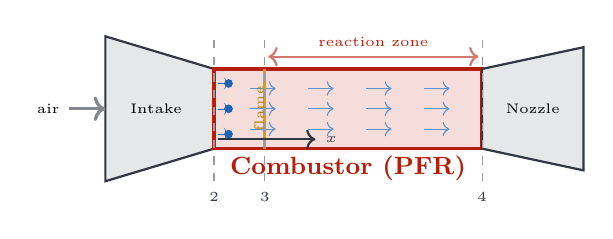
\begin{tikzpicture}[font=\small, scale=0.92]
    % ── Ramjet cross-section ──────────────────────────────────────────
    % Intake (converging)
    \draw[thick,ashgrey,fill=ashgrey!12]
      (0,1.0) -- (1.5,0.55) -- (1.5,-0.55) -- (0,-1.0) -- cycle;
    \node[font=\tiny] at (0.7,0) {Intake};

    % Combustor duct -- highlighted as PFR
    \draw[very thick,firered,fill=firered!15]
      (1.5,0.55) -- (5.2,0.55) -- (5.2,-0.55) -- (1.5,-0.55) -- cycle;
    % Flow direction arrows inside duct
    \foreach \xx in {2.0, 2.8, 3.6, 4.4}{
      \draw[->,skyblue!70,thin] (\xx,-0.28) -- (\xx+0.35,-0.28);
      \draw[->,skyblue!70,thin] (\xx, 0.00) -- (\xx+0.35, 0.00);
      \draw[->,skyblue!70,thin] (\xx, 0.28) -- (\xx+0.35, 0.28);
    }
    % Flame front / reaction zone
    \draw[very thick,flameyellow] (2.2,-0.55) -- (2.2,0.55);
    \node[font=\tiny,flameyellow!80!black,rotate=90] at (2.12,0) {flame};
    % Fuel injectors
    \foreach \yy in {0.35, 0.0, -0.35}{
      \fill[skyblue] (1.7,\yy) circle (0.06);
      \draw[->,skyblue,very thin] (1.55,\yy) -- (1.72,\yy);
    }
    \node[firered,font=\small\bfseries] at (3.35,-0.82) {Combustor (PFR)};

    % Nozzle
    \draw[thick,ashgrey,fill=ashgrey!12]
      (5.2,0.55) -- (6.6,0.85) -- (6.6,-0.85) -- (5.2,-0.55) -- cycle;
    \node[font=\tiny] at (5.9,0) {Nozzle};

    % Station labels
    \foreach \x/\lab in {1.5/2, 2.2/3, 5.2/4}{
      \draw[dashed,ashgrey!50,thin] (\x,-1.0) -- (\x,0.98);
      \node[below,font=\tiny,ashgrey] at (\x,-1.02) {\lab};
    }
    \draw[->,very thick,ashgrey!60] (-0.5,0) -- (0,0);
    \node[left,font=\tiny] at (-0.5,0) {air};

    % PFR label with brace
    \draw[<->,thick,firered!60] (2.25,0.72) -- (5.15,0.72)
      node[midway,above,font=\tiny,firered]{reaction zone};

    % x-axis arrow inside duct
    \draw[->,thick,ashgrey] (1.55,-0.42) -- (2.9,-0.42)
      node[right,font=\tiny]{$x$};
  \end{tikzpicture}
  \end{center}

  \medskip
  \begin{columns}
    \begin{column}{0.32\textwidth}
      \textbf{Ramjet combustor}\\
      Subsonic flow, $\Ma \approx 0.3$\\
      $L_c \sim 0.5$--$1.0$ m\\
      Spatial gradients matter
    \end{column}
    \begin{column}{0.32\textwidth}
      \textbf{Scramjet combustor}\\
      Supersonic flow, $\Ma > 1$\\
      $L_c \sim 0.3$--$0.8$ m\\
      Residence time $\sim 1$ ms
    \end{column}
    \begin{column}{0.32\textwidth}
      \textbf{Rocket thrust chamber}\\
      Near-stoichiometric\\
      High $p$, short $L_c$\\
      Axial profiles essential
    \end{column}
  \end{columns}
\end{frame}

\begin{frame}{WSR vs.\ PFR: When Does Spatial Structure Matter?}

  \begin{columns}
    \begin{column}{0.50\textwidth}
      \begin{block}{WSR (recall)}
        \begin{itemize}
          \item \textbf{Zero-dimensional}: $\nabla \equiv \mathbf{0}$
          \item Instantaneous mixing; uniform $T$, $Y_k$ throughout
          \item Governs: main combustor primary zone,
                jet-stirred lab reactors
          \item Key output: extinction/blowout limits, $\eta_c$
        \end{itemize}
      \end{block}
    \end{column}
    \begin{column}{0.46\textwidth}
      \begin{alertblock}{PFR (this lecture)}
        \begin{itemize}
          \item \textbf{One-dimensional}: gradients only along $x$
          \item No mixing \emph{across} streamlines; plug velocity profile
          \item Governs: ramjet/scramjet ducts, afterburner
                downstream zone, rocket chambers
          \item Key outputs: $T(x)$, $Y_k(x)$, ignition length,
                burnout length
        \end{itemize}
      \end{alertblock}
    \end{column}
  \end{columns}

 % \medskip
  \begin{exampleblock}{Rule of thumb for aero-combustors}
    Use WSR when $t_{\text{mix}} \ll \tchem$; use PFR when
    $t_{\text{mix}} \gg \tchem$ or when the flow has a strong axial
 directionality (ducts, nozzles, ramjet/scramjet passages).
  \end{exampleblock}
\end{frame}

% ════════════════════════════════════════════════════════════════════════
\section{The One-Dimensional Idealization}
% ════════════════════════════════════════════════════════════════════════

\begin{frame}{The Plug Flow Idealization}

  \begin{columns}
    \begin{column}{0.55\textwidth}
      A \textbf{Plug Flow Reactor (PFR)} retains \emph{one} spatial
      dimension (the axial coordinate $x$) and discards all others:
      \[
        \phi(x, r, \theta, t) \equiv \phi(x) \qquad \text{(steady state)}
      \]

      \begin{block}{Plug flow assumptions}
        \begin{enumerate}
          \item Uniform axial velocity profile: $u = u(x)$ only
          \item No radial or circumferential gradients
          \item No axial diffusion (convection $\gg$ diffusion):
                $Pe = uL/D \gg 1$
          \item Steady state: $\partial/\partial t = 0$
        \end{enumerate}
      \end{block}
    \end{column}
    \begin{column}{0.42\textwidth}
      \centering
      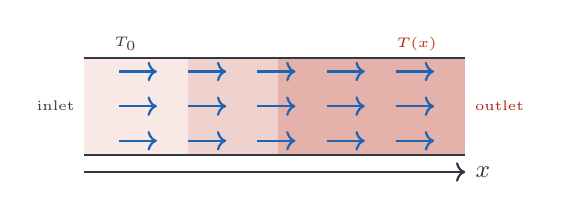
\begin{tikzpicture}[scale=0.88, font=\small]
        % Duct outline
        \draw[thick,ashgrey] (0,0.7) -- (5.5,0.7);
        \draw[thick,ashgrey] (0,-0.7) -- (5.5,-0.7);
        % Flat velocity profiles (plug flow)
        \foreach \xx in {0.5, 1.5, 2.5, 3.5, 4.5}{
          \draw[->,skyblue,thick] (\xx,-0.5) -- (\xx+0.55,-0.5);
          \draw[->,skyblue,thick] (\xx, 0.0) -- (\xx+0.55, 0.0);
          \draw[->,skyblue,thick] (\xx, 0.5) -- (\xx+0.55, 0.5);
        }
        % Colour gradient (cold to hot)
        \fill[firered!10] (0,-0.7) rectangle (5.5,0.7);
        \fill[firered!30,opacity=0.5] (1.5,-0.7) rectangle (5.5,0.7);
        \fill[firered!55,opacity=0.4] (2.8,-0.7) rectangle (5.5,0.7);
        % Redraw walls on top
        \draw[thick,ashgrey] (0,0.7) -- (5.5,0.7);
        \draw[thick,ashgrey] (0,-0.7) -- (5.5,-0.7);
        \foreach \xx in {0.5, 1.5, 2.5, 3.5, 4.5}{
          \draw[->,skyblue,thick] (\xx,-0.5) -- (\xx+0.55,-0.5);
          \draw[->,skyblue,thick] (\xx, 0.0) -- (\xx+0.55, 0.0);
          \draw[->,skyblue,thick] (\xx, 0.5) -- (\xx+0.55, 0.5);
        }
        % x axis
        \draw[->,thick,ashgrey] (0,-0.95) -- (5.5,-0.95)
          node[right]{$x$};
        \node[left,font=\tiny,ashgrey] at (0,0) {inlet};
        \node[right,font=\tiny,firered] at (5.5,0) {outlet};
        % Temperature label
        \node[font=\tiny,ashgrey] at (0.6,0.9) {$T_0$};
        \node[font=\tiny,firered] at (4.8,0.9) {$T(x)$};
      \end{tikzpicture}
      \vspace{0.2em}

      \small Flat velocity profiles; $T$ and $Y_k$ vary \emph{only} with $x$.
    \end{column}
  \end{columns}
\end{frame}

\begin{frame}{What the 1-D Assumption Eliminates and Retains}

  \begin{columns}[t]
    \begin{column}{0.48\textwidth}
      \textbf{Full reactive Navier--Stokes}
      \begin{align*}
        \rho\left(\pd{u_i}{t} + u_j\pd{u_i}{x_j}\right)
          &= -\pd{p}{x_i} + \ldots\\
        \rho\pd{Y_k}{t} + \rho u_j\pd{Y_k}{x_j}
          &= \nabla\cdot(\rho D_k\nabla Y_k) + \wdot_k W_k\\
        \rho c_p\pd{T}{t} + \rho c_p u_j\pd{T}{x_j}
          &= \nabla\cdot(\lambda\nabla T) - \textstyle\sum_k h_k\wdot_k W_k
      \end{align*}
    \end{column}
    \begin{column}{0.48\textwidth}
      \textbf{1-D PFR \quad ($\partial/\partial r = \partial/\partial\theta = 0$,
      $Pe \gg 1$)}
      \begin{align*}
        \rho u \ddx{Y_k}
          &= \wdot_k W_k \\[8pt]
        \rho u c_p \ddx{T}
          &= -\sum_k h_k \wdot_k W_k \\[8pt]
        \ddx{(\rho u)}
          &= 0 \quad \text{(continuity)}
      \end{align*}
    \end{column}
  \end{columns}

  \medskip
  \begin{block}{What is retained compared to the WSR}
    \begin{itemize}
      \item The \textbf{axial derivative} $d/dx$ --- spatial structure
            along the flow direction is fully resolved.
      \item The \textbf{convective transport} term $\rho u\,d(\cdot)/dx$
            replaces the residence-time flux $(\cdot_{\text{in}} - \cdot)/\tau$
            of the WSR.
    \end{itemize}
  \end{block}
\end{frame}

% ════════════════════════════════════════════════════════════════════════
\section{Governing Equations}
% ════════════════════════════════════════════════════════════════════════

\begin{frame}{Species Conservation in a PFR}

  Consider a control volume of cross-sectional area $\Ac$ and width
  $dx$ at position $x$. Species $k$ balance:
  \[
    \underbrace{\rho u \Ac \, Y_k\big|_x}_{\text{in}}
    - \underbrace{\rho u \Ac \, Y_k\big|_{x+dx}}_{\text{out}}
    + \underbrace{\wdot_k W_k \Ac\,dx}_{\text{production}}
    = 0
  \]

  Dividing by $\Ac\,dx$ and taking $dx\to 0$:
  \[
    \boxed{
      \rho u \ddx{Y_k} = \wdot_k W_k
    }
  \]

  \begin{itemize}
    \item $\wdot_k$ --- net molar production rate of species $k$
          (mol~m$^{-3}$~s$^{-1}$), evaluated at \alert{local} $(T, p, Y_k)$.
    \item Unlike the WSR, rates are \emph{not} fixed at exit conditions ---
          they vary continuously along $x$.
    \item System of $N_{\text{spec}}$ coupled first-order ODEs in $x$.
  \end{itemize}
\end{frame}

\begin{frame}{Energy Conservation in a PFR}

  For a steady, adiabatic, low-Mach PFR at constant pressure:
  \[
    \boxed{
      \rho u c_p \ddx{T} = -\sum_{k=1}^{N} h_k \wdot_k W_k
    }
  \]

  \begin{columns}[t]
    \begin{column}{0.50\textwidth}
      \textbf{Compact form using heat release}\\[4pt]
      Define the volumetric heat release rate:
      \[
        \dot{q}''' = -\sum_k h_k \wdot_k W_k > 0
        \quad\text{(exothermic)}
      \]
      Then:
      \[
        \ddx{T} = \frac{\dot{q}'''}{\rho u c_p}
      \]
      Temperature rises wherever $\dot{q}''' > 0$.
    \end{column}
    \begin{column}{0.46\textwidth}
      \textbf{With wall heat loss}\\[4pt]
      For a combustor with perimeter $P_w$ and
      wall heat flux $q_w''$ (W~m$^{-2}$):
      \[
        \rho u c_p \ddx{T}
        = \dot{q}''' - \frac{P_w q_w''}{\Ac}
      \]
      \small Relevant for cooled rocket chambers
      and film-cooled scramjet liners.
    \end{column}
  \end{columns}
\end{frame}

\begin{frame}{Continuity and Momentum}

  \textbf{Continuity} (mass conservation along $x$):
  \[
    \ddx{(\rho u \Ac)} = 0
    \quad\Rightarrow\quad
    \mdot = \rho u \Ac = \text{const}
  \]
  For constant-area duct ($\Ac = \text{const}$):
  $\rho u = \text{const}$, i.e.\ density and velocity trade off
  as combustion heats the gas.

  \medskip
  \textbf{Momentum} (low-Mach, negligible friction):
  \[
    p \approx \text{const}
    \quad\Rightarrow\quad
    \rho = \frac{p\bar{W}}{R_u T} \propto \frac{1}{T}
  \]
  So velocity increases with temperature:
  \[
    u(x) = \frac{\mdot}{\rho(x)\Ac} = \frac{\mdot R_u T(x)}{p \bar{W}(x) \Ac}
  \]

  \begin{alertblock}{Gas expansion in an aero-combustor}
    For $T$ rising from 700~K to 2000~K, $u$ nearly triples.
    This \textbf{thermal choking} limits the combustor inlet Mach number
    and is a central design constraint in ramjet combustors.
  \end{alertblock}
\end{frame}

\begin{frame}{Residence Time and the Damkohler Number}

  Unlike the WSR (where $\tau = \rho V / \mdot$ is a global parameter),
  the PFR has a \textbf{local residence time}:
  \[
    t(x) = \int_0^x \frac{dx'}{u(x')}
    = \int_0^x \frac{\rho(x')\Ac}{\mdot}\,dx'
  \]

  \begin{block}{PFR residence time to the exit}
    \[
      \taupfr = \int_0^{L_c} \frac{dx}{u(x)}
      = \frac{\Ac}{\mdot}\int_0^{L_c}\rho(x)\,dx
    \]
    For constant-area, ideal gas at constant $p$:
    $\taupfr \approx L_c\bar\rho / (\mdot/\Ac)$
    where $\bar\rho$ is the mean density.
  \end{block}

  \medskip
  The \textbf{local Damkohler number} varies along $x$:
  \[
    \Da(x) = \frac{t(x)}{\tchem(x)}
    \qquad
    \tchem(x) = \frac{\rho Y_{F}}{\wdot_F W_F}\bigg|_x
  \]
  Combustion is complete when $\Da(L_c) \gg 1$.
\end{frame}

% ════════════════════════════════════════════════════════════════════════
\section{Analytical Solutions}
% ════════════════════════════════════════════════════════════════════════

\begin{frame}{First-Order Reaction: Exact Solution}

  For a single-step reaction with $-\wdot_F W_F = k(T)\rho Y_F$
  (first order in fuel, $k = Ae^{-E_a/R_u T}$):
  \[
    \rho u \ddx{Y_F} = -k\rho Y_F
    \quad\Rightarrow\quad
    \ddx{Y_F} = -\frac{k}{u} Y_F
  \]

  For an \textbf{isothermal} PFR (or frozen-chemistry approximation):
  \[
    Y_F(x) = Y_{F,0}\,\exp\!\left(-\frac{kx}{u}\right)
    = Y_{F,0}\,\exp\!\left(-k\,t(x)\right)
    = Y_{F,0}\,e^{-\Da(x)}
  \]

  \begin{columns}[t]
    \begin{column}{0.50\textwidth}
      \textbf{Conversion vs.\ Damkohler number}
      \[
        X_F(x) = 1 - e^{-\Da(x)}
      \]
      \begin{itemize}
        \item $\Da = 1$: $X_F = 63\%$
        \item $\Da = 3$: $X_F = 95\%$
        \item $\Da = 5$: $X_F = 99.3\%$
      \end{itemize}
    \end{column}
    \begin{column}{0.46\textwidth}
      \textbf{Compare to WSR (1st order)}
      \[
        X_F^{\text{WSR}} = \frac{\Da}{1+\Da}
      \]
      \begin{itemize}
        \item $\Da = 1$: $X_F^{\text{WSR}} = 50\%$
        \item $\Da = 3$: $X_F^{\text{WSR}} = 75\%$
        \item PFR always \emph{more efficient} than WSR
      \end{itemize}
    \end{column}
  \end{columns}
\end{frame}

\begin{frame}{PFR vs.\ WSR Efficiency: Levenspiel Comparison}

  \centering
  \begin{tikzpicture}
    \begin{axis}[
        width=0.82\textwidth, height=0.60\textheight,
        xlabel={Damkohler number $\Da = k\tau$},
        ylabel={Fuel conversion $X_F$},
        xmin=0, xmax=5.5, ymin=0, ymax=1.05,
        samples=200, domain=0:5.4,
        grid=major, thick,
        legend pos=south east,
        legend style={font=\small},
    ]
      \addplot[firered, very thick] {1 - exp(-x)};
      \addlegendentry{PFR: $1-e^{-\Da}$}
      \addplot[skyblue, very thick, dashed] {x/(1+x)};
      \addlegendentry{WSR: $\Da/(1+\Da)$}
      % Annotate at Da=2
      \draw[dotted,ashgrey] (axis cs:2,0) -- (axis cs:2,0.865);
      \draw[dotted,ashgrey] (axis cs:2,0) -- (axis cs:2,0.667);
      \node[right,font=\tiny,firered] at (axis cs:2.05,0.865)
        {PFR 86.5\%};
      \node[right,font=\tiny,skyblue] at (axis cs:2.05,0.667)
        {WSR 66.7\%};
    \end{axis}
  \end{tikzpicture}

  \small For the \emph{same} $\Da$ (i.e.\ same combustor volume and
  flow conditions), the PFR always achieves higher fuel conversion.
  At $\Da=2$: PFR gives 87\% vs.\ WSR 67\%.
\end{frame}

\begin{frame}{Adiabatic Temperature Profile}

  For a global one-step reaction in an adiabatic PFR:
  \[
    T(x) = T_0 + \frac{Q_{\text{HV}}}{c_p}\bigl(Y_{F,0} - Y_F(x)\bigr)
    = T_0 + \Delta T_{\text{ad}}\,X_F(x)
  \]

  \begin{columns}
    \begin{column}{0.50\textwidth}
      \centering
      \begin{tikzpicture}
        \begin{axis}[
            width=\textwidth, height=0.55\textheight,
            xlabel={$x/L_c$},
            ylabel={$T$ (normalised)},
            xmin=0, xmax=1.05, ymin=0, ymax=1.05,
            samples=150, domain=0:1,
            grid=major, thick,
            ytick={0.2,0.6,1.0},
            yticklabels={$T_0$, $T_0+0.6\Delta T_{\text{ad}}$, $\Tad$},
            xtick={0,0.5,1.0},
        ]
          % Temperature profile for Da=3 over unit length
          % X_F(x) = 1-exp(-3x), T norm = 0.2 + 0.8*(1-exp(-3x))
          \addplot[firered, very thick]
            {0.2 + 0.8*(1-exp(-3*x))};
          \addplot[ashgrey, dashed]
            coordinates{(0,0.2)(1,0.2)};
          \node[right,font=\tiny,ashgrey] at (axis cs:0.02,0.17)
            {$T_0$};
          \addplot[ashgrey, dashed]
            coordinates{(0,1.0)(1,1.0)};
          \node[right,font=\tiny,ashgrey] at (axis cs:0.02,1.03)
            {$\Tad$};
        \end{axis}
      \end{tikzpicture}
    \end{column}
    \begin{column}{0.46\textwidth}
      \begin{itemize}
        \item $T$ rises steeply where $\wdot_F$ is large (hot zone)
        \item Asymptotes to $\Tad$ as $Y_F \to 0$
        \item For Arrhenius kinetics: initial slow rise
              (cold inlet), then rapid acceleration (thermal runaway
              in the positive sense), then plateau
        \item This \textbf{S-shape in $T(x)$} is characteristic
              of all adiabatic combustion PFRs
      \end{itemize}
    \end{column}
  \end{columns}
\end{frame}

% ════════════════════════════════════════════════════════════════════════
\section{Ignition Length and Burnout Length}
% ════════════════════════════════════════════════════════════════════════

\begin{frame}{Ignition Length in a PFR}

  A critical aero-propulsion quantity: \textbf{how far downstream
  does combustion begin?}

  \medskip
  For Arrhenius kinetics, the initial cold-flow region has negligible
  reaction.  The \textbf{ignition length} $x_{\text{ign}}$ is the
  axial location where the temperature first rises sharply:
  \[
    x_{\text{ign}} \approx \frac{u_0}{\rho_0 / \tchem(T_0)}
    = u_0 \tchem(T_0)
  \]

  A more useful estimate using the crossover temperature $T^*$
  (where $\dot{q}''' > \dot{q}'''_{\text{loss}}$):
  \[
    x_{\text{ign}} \approx \int_0^{t^*} u(t)\,dt
    \quad\text{where}\quad
    t^* = \frac{c_p(T^* - T_0)}{Q_{\text{HV}}\,\wdot_F(T^*)/\rho}
  \]

  \begin{alertblock}{Scramjet ignition crisis}
    In a scramjet ($u \sim 1500$--$3000$ m/s, $L_c \sim 0.5$ m),
    the available residence time is $\taupfr \sim 0.1$--$0.3$ ms.
    If $x_{\text{ign}} > L_c$, the fuel exits unburned.
    This drives the use of \textbf{radical enhancers} (H$_2$ pilots)
    and \textbf{cavity flameholders} to reduce $\tchem$.
  \end{alertblock}
\end{frame}

\begin{frame}{Burnout Length}

  The \textbf{burnout length} $x_{\text{bo}}$ is where fuel conversion
  reaches a specified level (e.g.\ $X_F = 0.999$):
  \[
    x_{\text{bo}} : \quad Y_F(x_{\text{bo}}) = (1 - 0.999)\,Y_{F,0}
  \]

  For first-order kinetics at constant $T$ (isothermal approximation):
  \[
    x_{\text{bo}} = \frac{u}{k}\ln\frac{1}{0.001}
    = \frac{6.9\,u}{k}
    = \frac{6.9\,u}{A\,e^{-E_a/R_u T}}
  \]

  \begin{columns}[t]
    \begin{column}{0.50\textwidth}
      \textbf{Ramjet ($p=3$ bar, $T=1800$ K)}\\
      $k \sim 10^4$~s$^{-1}$ (Jet-A global)\\
      $u \sim 120$ m/s\\
      $x_{\text{bo}} \approx 0.08$ m --- achievable
    \end{column}
    \begin{column}{0.46\textwidth}
      \textbf{Scramjet ($p=1$ bar, $T=1400$ K)}\\
      $k \sim 10^3$~s$^{-1}$\\
      $u \sim 2000$ m/s\\
      $x_{\text{bo}} \approx 14$ m --- \alert{not achievable!}\\
      $\Rightarrow$ cavity/pilot essential
    \end{column}
  \end{columns}

  \begin{exampleblock}{Design implication}
    Burnout length $x_{\text{bo}} \propto u/k \propto u\,e^{+E_a/R_u T}/A$.
    Higher inlet temperature (higher $\Ma$) reduces $\tchem$ and
    therefore $x_{\text{bo}}$, partially offsetting the velocity increase.
  \end{exampleblock}
\end{frame}

% ════════════════════════════════════════════════════════════════════════
\section{Thermal Choking and Compressible PFR}
% ════════════════════════════════════════════════════════════════════════

\begin{frame}{Rayleigh Flow: Heat Addition to Compressible Flow}

  When the low-Mach approximation breaks down (e.g.\ ramjet
  combustor inlet $\Ma > 0.2$, scramjet), we must account for
  the coupling of heat addition and Mach number.

  \medskip
  For \textbf{Rayleigh flow} (constant-area duct, heat addition $\delta q$,
  no friction):
  \[
    \frac{dT_t}{T_t} = \frac{1 + \gamma\Ma^2}{1-\Ma^2}
    \cdot \frac{dT_t}{T_t}
    \qquad\text{(from Rayleigh relations)}
  \]

  The Mach number evolves as:
  \[
    \frac{d\Ma^2}{dx}
    = \frac{\Ma^2(1+\frac{\gamma-1}{2}\Ma^2)}{1-\Ma^2}
      \cdot \frac{2\dot{q}'''}{c_p T_t \rho u}
  \]

  \begin{alertblock}{Thermal choking ($\Ma \to 1$)}
    Heat addition drives subsonic flow towards $\Ma = 1$ and
    supersonic flow \emph{also} towards $\Ma = 1$ (from above).
    Adding more heat once $\Ma = 1$ is reached causes an
    \textbf{unstart} (normal shock ingested into intake) ---
    a critical structural failure mode in ramjets.
  \end{alertblock}
\end{frame}

\begin{frame}{Maximum Heat Addition Before Thermal Choking}

  From Rayleigh relations, the maximum total temperature ratio
  from inlet $\Ma_1$ to the choked exit ($\Ma_2 = 1$):
  \[
    \frac{T_{t,\text{max}}}{T_{t,1}}
    = \frac{(1+\gamma)^2 \Ma_1^2}{(1+\gamma\Ma_1^2)^2}
    \cdot \frac{1}{1} \quad (\text{Rayleigh, } \Ma_2=1)
  \]

  \begin{columns}
    \begin{column}{0.52\textwidth}
      \centering
      \begin{tikzpicture}
        \begin{axis}[
            width=\textwidth, height=0.52\textheight,
            xlabel={Inlet Mach $\Ma_1$},
            ylabel={$T_{t,\text{max}}/T_{t,1}$ (choking ratio)},
            xmin=0.1, xmax=2.0, ymin=0.9, ymax=4.5,
            samples=200, domain=0.15:1.95,
            grid=major, thick,
            legend pos=north east, legend style={font=\tiny},
        ]
          % Rayleigh Tt ratio to choking (gamma=1.3)
          % Tt2/Tt1 = (1+gamma)^2*Ma1^2 / (1+gamma*Ma1^2)^2
          \addplot[firered,very thick]
            {(1+1.3)^2 * x^2 / (1+1.3*x^2)^2};
          \addlegendentry{$\gamma=1.3$ (hot gas)}
          \addplot[skyblue,thick,dashed]
            {(1+1.4)^2 * x^2 / (1+1.4*x^2)^2};
          \addlegendentry{$\gamma=1.4$ (cold)}
          % Choke line
          \addplot[ashgrey,dotted]
            coordinates{(0.1,1)(2.0,1)};
          \node[right,font=\tiny,ashgrey] at (axis cs:0.15,1.05)
            {no heat can be added};
          \draw[dotted,ashgrey] (axis cs:1.0,0.9)--(axis cs:1.0,4.5);
        \end{axis}
      \end{tikzpicture}
    \end{column}
    \begin{column}{0.44\textwidth}
      \begin{itemize}
        \item At $\Ma_1 = 0.3$: $T_t$ can increase $\approx 3.5\times$
              before choking (typical ramjet: safe)
        \item At $\Ma_1 = 0.7$: margin shrinks considerably
        \item Supersonic ($\Ma_1 > 1$): choking drives $\Ma \to 1$
              from above; \emph{very} sensitive
        \item Scramjet designers must keep heat release
              distributed to avoid local $\Ma \to 1$
      \end{itemize}
    \end{column}
  \end{columns}
\end{frame}

% ════════════════════════════════════════════════════════════════════════
\section{PFR in Aerospace Applications}
% ════════════════════════════════════════════════════════════════════════

\begin{frame}{Ramjet Combustor Design Using PFR Model}

  \begin{columns}[t]
    \begin{column}{0.52\textwidth}
      \textbf{Design problem}\\[4pt]
      Given: $p_3$, $T_3$, $\Ma_3$, $\phi$, fuel = Jet-A\\
      Find: required combustor length $L_c$ for $\eta_c \geq 0.99$

      \medskip
      \textbf{Procedure (PFR method):}
      \begin{enumerate}
        \item Set inlet: $\rho_0 = p_3\bar{W}/(R_u T_3)$,
              $u_0 = \Ma_3 \sqrt{\gamma R T_3}$
        \item Integrate ODEs:
              $\rho u dY_F/dx = \wdot_F W_F$,
              $\rho u c_p dT/dx = \dot{q}'''$
        \item Update $\rho(x) = p\bar{W}(x)/(R_u T(x))$,
              $u(x) = \mdot / (\rho \Ac)$ at each step
        \item Stop when $Y_F < 0.01 Y_{F,0}$
      \end{enumerate}
    \end{column}
    \begin{column}{0.44\textwidth}
      \begin{exampleblock}{Typical ramjet numbers}
        \begin{tabular}{lc}
          $p_3$ & 3 bar \\
          $T_3$ & 800 K \\
          $\Ma_3$ & 0.25 \\
          $\phi$ & 0.9 \\
          $u_0$ & $\sim 180$ m/s \\
          $\taupfr$ & $\sim 4$ ms \\
          $L_c$ & $\sim 0.7$ m \\
        \end{tabular}
      \end{exampleblock}
      \medskip
      The PFR gives $T(x)$, $Y_k(x)$, and $\Ma(x)$
      profiles in one integration pass ---
      far more information than the WSR scalar output.
    \end{column}
  \end{columns}
\end{frame}

\begin{frame}{Scramjet Combustor: Supersonic PFR}

  In a scramjet, $\Ma_3 > 1$ and combustion occurs in supersonic
  flow.  The PFR equations are unchanged but the Rayleigh coupling
  is now critical.

  \begin{columns}[t]
    \begin{column}{0.54\textwidth}
      \textbf{Key differences from subsonic PFR}
      \begin{itemize}
        \item $\Ma > 1$: pressure gradient and velocity gradient
              have \emph{opposite} signs to subsonic case
        \item Heat addition \emph{decelerates} supersonic flow
              ($u$ decreases, $\rho$ increases slightly)
        \item Static temperature rises --- beneficial for kinetics
        \item Auto-ignition delay can be expressed as an
              \textbf{ignition length} at the supersonic flow speed
        \item If $x_{\text{ign}} > L_c$: unburned fuel in nozzle
      \end{itemize}
    \end{column}
    \begin{column}{0.42\textwidth}
      \begin{alertblock}{Scramjet ignition numbers}
        $Ma_3 = 2.5$, $T_3 = 1200$ K, $p_3 = 0.8$ bar\\
        $u_3 \approx 1750$ m/s\\
        $\tchem \approx 0.5$ ms (H$_2$)\\
        \hspace{1.8em} $\approx 5$ ms (kerosene)\\[4pt]
        $x_{\text{ign,H}_2} \approx 0.9$ m\\
        $x_{\text{ign,kero}} \approx 8.7$ m
      \end{alertblock}
      \small Hydrogen is the only practical scramjet fuel
      for $\Ma > 8$ flight; kerosene requires radical-assisted
      ignition below $\Ma \approx 10$.
    \end{column}
  \end{columns}
\end{frame}

\begin{frame}{Afterburner as a PFR}

The afterburner operates downstream of the turbine: the flow is
axial, hot (800--1000 K), and at low pressure (2--5 bar). 

   \begin{itemize}
        \item The \emph{far-field} region downstream of the
              V-gutter flameholder behaves as a plug-flow zone
        \item The \emph{near-field} recirculation zone is
             modelled as a WSR 
        \item Combined WSR-PFR model: recirculation provides
              hot products to ignite the PFR mainstream
        \item Burnout length $x_{\text{bo}}$ sets the
              minimum afterburner duct length
      \end{itemize}

\end{frame}

% ════════════════════════════════════════════════════════════════════════
\section{WSR--PFR Comparison and Series Networks}
% ════════════════════════════════════════════════════════════════════════

\begin{frame}{WSR vs.\ PFR: Head-to-Head Summary}

  \renewcommand{\arraystretch}{1.5}
  \begin{tabular}{>{\bfseries}p{3.2cm} p{4.5cm} p{4.5cm}}
    \toprule
    Property & WSR (Unit 4) & PFR (this unit) \\
    \midrule
    Dimensionality & 0-D: $\nabla \equiv \mathbf{0}$ &
                     1-D: $d/dx \neq 0$ \\
    Governing eqns & Algebraic (steady state) &
                     ODEs in $x$ \\
    Mixing model   & Perfect, instantaneous &
                     No radial mixing; plug flow \\
    Rate evaluation & At \emph{exit} (hot) state &
                     At \emph{local} $T(x)$, $Y_k(x)$ \\
    Efficiency ($n>0$) & Lower for same $\Da$ &
                     Higher for same $\Da$ \\
    Key limit      & Blowout ($\Da \to 1$) &
                     Burnout length, ignition length \\
    Propulsion use & Primary zone, JSR lab &
                     Ramjet, scramjet, afterburner PFR zone \\
    \bottomrule
  \end{tabular}
\end{frame}

\begin{frame}{WSR--PFR Series Network}

  Real combustors are often modelled as a \textbf{WSR followed by
  a PFR}: the recirculation zone (WSR) stabilises the flame and
  the mainstream duct (PFR) completes burnout.

  \medskip
  \begin{center}
  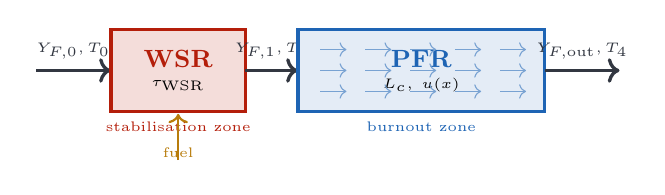
\begin{tikzpicture}[font=\small, scale=0.95]
    % Inlet arrow
    \draw[->,very thick,ashgrey] (0,0) -- (1.0,0)
      node[midway,above,font=\tiny]{$Y_{F,0},T_0$};
    % WSR box
    \draw[very thick,firered,fill=firered!15]
      (1.0,-0.55) rectangle (2.8,0.55);
    \node[font=\small\bfseries,firered] at (1.9,0.15) {WSR};
    \node[font=\tiny] at (1.9,-0.2) {$\tau_{\text{WSR}}$};
    % Arrow WSR to PFR
    \draw[->,very thick,ashgrey] (2.8,0) -- (3.5,0)
      node[midway,above,font=\tiny]{$Y_{F,1},T_1$};
    % PFR box
    \draw[very thick,skyblue,fill=skyblue!12]
      (3.5,-0.55) rectangle (6.8,0.55);
    \node[font=\small\bfseries,skyblue] at (5.15,0.15) {PFR};
    \node[font=\tiny] at (5.15,-0.2) {$L_c,\;u(x)$};
    % Flow arrows inside PFR
    \foreach \xx in {3.8,4.4,5.0,5.6,6.2}{
      \draw[->,thin,skyblue!60] (\xx,0.28)--(\xx+0.35,0.28);
      \draw[->,thin,skyblue!60] (\xx,0.00)--(\xx+0.35,0.00);
      \draw[->,thin,skyblue!60] (\xx,-0.28)--(\xx+0.35,-0.28);
    }
    % Outlet arrow
    \draw[->,very thick,ashgrey] (6.8,0) -- (7.8,0)
      node[midway,above,font=\tiny]{$Y_{F,\text{out}},T_4$};
    % Labels below
    \node[firered,font=\tiny] at (1.9,-0.75)
      {stabilisation zone};
    \node[skyblue,font=\tiny] at (5.15,-0.75)
      {burnout zone};
    % Fuel injection arrow into WSR
    \draw[->,thick,flameyellow!80!black] (1.9,-1.2) -- (1.9,-0.58)
      node[below,font=\tiny,flameyellow!80!black,yshift=-0.3cm]
      {fuel};
  \end{tikzpicture}
  \end{center}

  \medskip
  \begin{itemize}
    \item WSR output $(Y_{F,1}, T_1)$ becomes the PFR inlet condition.
    \item WSR sets the \textbf{blowout limit}; PFR sets the
          \textbf{burnout length}.
    \item This two-zone model is the standard preliminary design
          tool for afterburners and ramjet combustors.
  \end{itemize}
\end{frame}

% ════════════════════════════════════════════════════════════════════════
\section{Numerical Integration of the PFR}
% ════════════════════════════════════════════════════════════════════════

\begin{frame}{Numerical Method: Spatial Integration}

  The PFR ODE system at each step $x_n \to x_{n+1}$:
  \begin{align*}
    \frac{dY_k}{dx} &= \frac{\wdot_k W_k}{\rho u}, \quad k = 1,\ldots,N \\[6pt]
    \frac{dT}{dx}   &= \frac{-\sum_k h_k \wdot_k W_k}{\rho u c_p} \\[6pt]
    \rho(x)         &= \frac{p\bar{W}(T,Y_k)}{R_u T}, \quad
    u(x) = \frac{\mdot}{\rho\Ac}
  \end{align*}

  \begin{columns}[t]
    \begin{column}{0.50\textwidth}
      \textbf{Numerical considerations}
      \begin{itemize}
        \item System is \textbf{stiff} near the reaction zone
              ($d\wdot_k/dT$ very large via Arrhenius)
        \item Use implicit methods: CVODE (BDF), LSODA, Radau
        \item Adaptive step-size essential: $\Delta x$ can vary
              by $10^4$ across the domain
        \item Cantera \code{FreeFlame} or \code{IdealGasFlow}
              objects handle this automatically
      \end{itemize}
    \end{column}
    \begin{column}{0.46\textwidth}
      \textbf{Cantera implementation}
      \begin{itemize}
        \item \code{IdealGasFlow} reactor with
              \code{AxisymmetricFlow} or
              \code{FreeFlame} geometry
        \item Alternatively: \code{FlowReactor}
              for simple duct geometry
        \item State vector: $(T, Y_1, \ldots, Y_N)$
              indexed by axial position
        \item Post-process with
              \code{flame.T}, \code{flame.X[sp, :]}
      \end{itemize}
    \end{column}
  \end{columns}
\end{frame}

\begin{frame}{Modelling Hierarchy: Where PFR Fits}

  \renewcommand{\arraystretch}{1.35}
  \begin{tabular}{>{\bfseries}p{3.4cm} p{4.0cm} p{4.2cm}}
    \toprule
    Model & Computational cost & Propulsion use \\
    \midrule
    0-D WSR & $< 1$~s & Blowout/ignition limits,\\
             &          & fuel screening \\
    \alert{1-D PFR} & \alert{seconds} &
      \alert{Burnout/ignition length,}\\
      & & \alert{$T(x)$/$Y_k(x)$ profiles,}\\
      & & \alert{preliminary duct sizing} \\
    2-D axisymmetric & minutes & Swirl, recirculation zones \\
    3-D RANS CFD & hours & Full combustor aerodynamics \\
    LES / DNS & days--weeks & Instability, acoustics, soot \\
    \bottomrule
  \end{tabular}

  \medskip
  \begin{block}{PFR in the design cycle}
    After the WSR blowout map (Unit 4) selects a viable $(\phi, p, T_3)$
    operating point, the PFR is used to \textbf{size the combustor length}
    and verify burnout before committing to expensive CFD.
  \end{block}
\end{frame}

% ════════════════════════════════════════════════════════════════════════
\section{Summary}
% ════════════════════════════════════════════════════════════════════════

\begin{frame}{Key Equations at a Glance}
  \renewcommand{\arraystretch}{1.6}
  \begin{tabular}{>{\bfseries}p{4.0cm} p{7.4cm}}
    \toprule
    Concept & Expression \\
    \midrule
    PFR assumption & $\phi = \phi(x)$ only; no radial gradients,
                      $Pe \gg 1$ \\
    Species balance & $\rho u\,dY_k/dx = \wdot_k W_k$ \\
    Energy balance (adiab.) & $\rho u c_p\,dT/dx = -\sum_k h_k\wdot_k W_k$ \\
    Velocity (ideal gas) & $u(x) = \mdot R_u T(x)/(p\bar{W}\Ac)$ \\
    Residence time & $\taupfr = (\Ac/\mdot)\int_0^{L_c}\rho\,dx$ \\
    Local Da & $\Da(x) = t(x)/\tchem(x)$ \\
    Conversion (1st order, isothermal) & $X_F = 1 - e^{-\Da}$ \\
    Burnout length & $x_{\text{bo}} = 6.9\,u/k$ (isothermal, 1st order) \\
    Thermal choking & $d\Ma/dx \to \infty$ as $\Ma \to 1$ \\
    \bottomrule
  \end{tabular}
\end{frame}

\begin{frame}{Summary \& Take-Away Points}
  \begin{itemize}
    \item The PFR is a \textbf{one-dimensional} model: spatial
          structure along $x$ is retained, all radial/circumferential
          gradients are discarded. PDEs reduce to coupled ODEs in $x$.
    \item Unlike the WSR, reaction rates are evaluated at the
          \textbf{local} temperature and composition --- the PFR
          resolves the full evolution from cold inlet to hot products.
    \item For the same Damkohler number, the PFR always achieves
          \textbf{higher fuel conversion} than the WSR because it
          avoids back-mixing with cold inlet gas.
    \item The key design outputs are the \textbf{ignition length}
          $x_{\text{ign}}$ and \textbf{burnout length} $x_{\text{bo}}$,
          which directly set the required combustor duct length $L_c$.
    \item \alert{Thermal choking} (Rayleigh) limits heat addition in
          high-Mach combustors; this is a fundamental constraint for
          ramjet and scramjet design.
    \item In practice, combustors are modelled as a
          \textbf{WSR + PFR series network}: WSR governs blowout,
          PFR governs burnout length.
  \end{itemize}
  \vfill
\end{frame}

% ════════════════════════════════════════════════════════════════════════
% ════════════════════════════════════════════════════════════════════════
% Closing slide
% ════════════════════════════════════════════════════════════════════════
 
{
\setbeamertemplate{footline}{}
\setbeamertemplate{headline}{}
\setbeamercolor{background canvas}{bg=ashgrey}
\begin{frame}[plain, c]
 
  % Full-page dark background
  \begin{tikzpicture}[remember picture, overlay]
    \fill[ashgrey] (current page.south west)
                   rectangle (current page.north east);
    % Faint diagonal speed-line accents (bottom-left to mid)
    \foreach \ang/\op in {8/0.04, 6/0.03, 10/0.03}{
      \draw[white, line width=0.5pt, opacity=\op,
            rotate around={\ang:(current page.west)}]
        ([xshift=-1cm]current page.west)
        -- ([xshift=1cm]current page.east);
    }
    % Warm glow bottom-right corner (reaction zone suggestion)
    \fill[firered, opacity=0.12]
      (current page.south east) circle (4.5cm);
    \fill[flameyellow, opacity=0.07]
      (current page.south east) circle (2.5cm);
  \end{tikzpicture}
 
  % ── Title block ─────────────────────────────────────────────────────
  \vspace{0.55cm}
  {\color{white}\fontsize{22}{26}\selectfont\bfseries
   The Plug Flow Reactor}
 
  \vspace{0.10cm}
  {\color{skyblue!70}\fontsize{9}{11}\selectfont
    Combustion\enspace|\enspace
   UCK 427E}
 
  \vspace{0.12cm}
  % Two-tone rule: skyblue full width, firered left accent
  
\begin{tikzpicture}
    \draw[skyblue!60, line width=0.6pt] (0,0) -- (\textwidth,0);
    \draw[firered,    line width=2.2pt] (0,0) -- (0.28\textwidth,0);
  \end{tikzpicture}
 
  \vspace{0.30cm}
 
  % ── Three pillars ────────────────────────────────────────────────────
  \begin{columns}[t, totalwidth=\textwidth]
 
    \begin{column}{0.315\textwidth}
      \begin{beamercolorbox}[rounded=true, wd=\linewidth,
                             sep=6pt, center]{block title}
        \textbf{\small 1-D Idealisation}
      \end{beamercolorbox}
      \vspace{3pt}
      \begin{beamercolorbox}[rounded=true, wd=\linewidth,
                             sep=6pt, center]{block body}
        \color{ashgrey}\fontsize{7.5}{10}\selectfont
        $\phi=\phi(x)$ only; no radial gradients\\[3pt]
        Peclet number $Pe\gg 1$\\
        (no axial diffusion)\\[3pt]
        Full NS $\to$ ODE system in $x$
      \end{beamercolorbox}
    \end{column}
 
    \hfill
 
    \begin{column}{0.315\textwidth}
      \begin{beamercolorbox}[rounded=true, wd=\linewidth,
                             sep=6pt, center]{block title alerted}
        \textbf{\small Key Design Outputs}
      \end{beamercolorbox}
      \vspace{3pt}
      \begin{beamercolorbox}[rounded=true, wd=\linewidth,
                             sep=6pt, center]{block body alerted}
        \color{ashgrey}\fontsize{7.5}{10}\selectfont
        $T(x)$, $Y_k(x)$ profiles\\[3pt]
        Ignition length $x_{\text{ign}}$\\[3pt]
        Burnout length $x_{\text{bo}}$\\[3pt]
        Thermal choking margin
      \end{beamercolorbox}
    \end{column}
 
    \hfill
 
    \begin{column}{0.315\textwidth}
      \begin{beamercolorbox}[rounded=true, wd=\linewidth,
                             sep=6pt, center]{block title example}
        \textbf{\small Propulsion Context}
      \end{beamercolorbox}
      \vspace{3pt}
      \begin{beamercolorbox}[rounded=true, wd=\linewidth,
                             sep=6pt, center]{block body example}
        \color{black}\fontsize{7.5}{10}\selectfont
        Ramjet combustor sizing\\[3pt]
        Scramjet ignition analysis\\[3pt]
        Afterburner burnout zone\\[3pt]
        WSR\,+\,PFR series network
      \end{beamercolorbox}
    \end{column}
 
  \end{columns}
 
  \vspace{0.30cm}
 
  % ── Equation strip ───────────────────────────────────────────────────
  \begin{beamercolorbox}[rounded=true, wd=\textwidth,
                         sep=5pt, center]{block body}
    \color{skyblue!80}\fontsize{7.8}{10}\selectfont
    $\rho u\,\dfrac{dY_k}{dx} = \dot{\omega}_k W_k$
    \qquad\vrule width 0.4pt height 9pt depth 2pt\qquad
    $\rho u c_p\,\dfrac{dT}{dx} = -\displaystyle\sum_k h_k\dot{\omega}_k W_k$
    \qquad\vrule width 0.4pt height 9pt depth 2pt\qquad
    $X_F = 1 - e^{-\mathrm{Da}}$
    \qquad\vrule width 0.4pt height 9pt depth 2pt\qquad
    $x_{\text{bo}} = \dfrac{6.9\,u}{k}$
  \end{beamercolorbox}
 
  \vspace{0.22cm}
 
  % ── Next lecture line ────────────────────────────────────────────────
  \begin{center}
    {\color{white!50}\fontsize{7.5}{9}\selectfont
     \textbf{Next:}\enspace Laminar Premixed Flames \& Flame Speed}
  \end{center}
 
\end{frame}
}

% ════════════════════════════════════════════════════════════════════════


\end{document}
